\documentclass[12pt,a4paper]{article}

\usepackage[a4paper,text={16.5cm,25.2cm},centering]{geometry}
\usepackage{lmodern}
\usepackage{amssymb,amsmath}
\usepackage{bm}
\usepackage{graphicx}
\usepackage{microtype}
\usepackage{hyperref}
\usepackage{minted}
\setlength{\parindent}{0pt}
\setlength{\parskip}{1.2ex}

\hypersetup
       {   pdfauthor = {  },
           pdftitle={  },
           colorlinks=TRUE,
           linkcolor=black,
           citecolor=blue,
           urlcolor=blue
       }






\begin{document}



Potenčna metoda


Iščemo lastni vektor matrike matrike A za največjo lastno vrednost.


\subsection{Invariantna mera za Markovsko verigo}

\begin{minted}[texcomments = true, mathescape, fontsize=\small, xleftmargin=0.5em]{julia}
P = [0.1 0.4 0.5;
     0 0.5 0.5;
     0.2 0 0.8]

using Vaje06
\end{minted}

Invariantna mera je lastni vektor za $P^T$ za lastno vrednost 1.


\begin{minted}[texcomments = true, mathescape, fontsize=\small, xleftmargin=0.5em]{julia}
p, lambda = potencna(P', ones(3))
p = p/sum(p)
\end{minted}
\begin{minted}[texcomments = true, mathescape, fontsize=\small, xleftmargin=0.5em, frame = leftline]{text}
Potenčna metoda se je končala po 21 korakih.
3-element Vector{Float64}:
 0.15873015872617383
 0.12698412699209677
 0.7142857142817293
\end{minted}

Invariantna mera za Markovsko verigo na 6 vozliščih. (Bipartitni graf)


\begin{minted}[texcomments = true, mathescape, fontsize=\small, xleftmargin=0.5em]{julia}
P = [0 0.3 0 0.4 0 0.3;
     0.1 0 0.2 0 0.7 0;
     0 0.5 0 0.2 0 0.3;
     0.4 0 0.2 0 0.4 0;
     0 0.5 0 0.2 0 0.3;
     0.4 0 0.2 0 0.4 0]

using LinearAlgebra
eigen(P')

p, lambda = potencna(P', rand(6))
p = p/sum(p)
\end{minted}
\begin{minted}[texcomments = true, mathescape, fontsize=\small, xleftmargin=0.5em, frame = leftline]{text}
"Potenčna mentolda ne konver|$\ensuremath{\dj}$|ira v 100 korakih."
\end{minted}

Premik $A - \ensuremath{\delta}I$ Če so $\ensuremath{\lambda}_1,...,\ensuremath{\lambda}_n$ lastne vrednosti matrike A, potem so $\ensuremath{\lambda}_1-\ensuremath{\delta},...,\ensuremath{\lambda}_n-\ensuremath{\delta}$ lastne vrednosti matrike $A - \ensuremath{\delta}I$


Če ima matrika A več različnih lastnih vrednosti, ki so po absolutni vrednosti največje, potem potenčna metoda ne konvergira za vsak Začetni približek. V prejšnem primeru je imela matrika lastne vrednosti 1 in -1. Problem rešimo s premikom.


\begin{minted}[texcomments = true, mathescape, fontsize=\small, xleftmargin=0.5em]{julia}
B = P + I

p,lambda = potencna(B',rand(6))

p = p/sum(p)

using Plots

scatter(p,title="Invariantna porazdelitev")
\end{minted}
\begin{minted}[texcomments = true, mathescape, fontsize=\small, xleftmargin=0.5em, frame = leftline]{text}
Potenčna metoda se je končala po 41 korakih.
\end{minted}
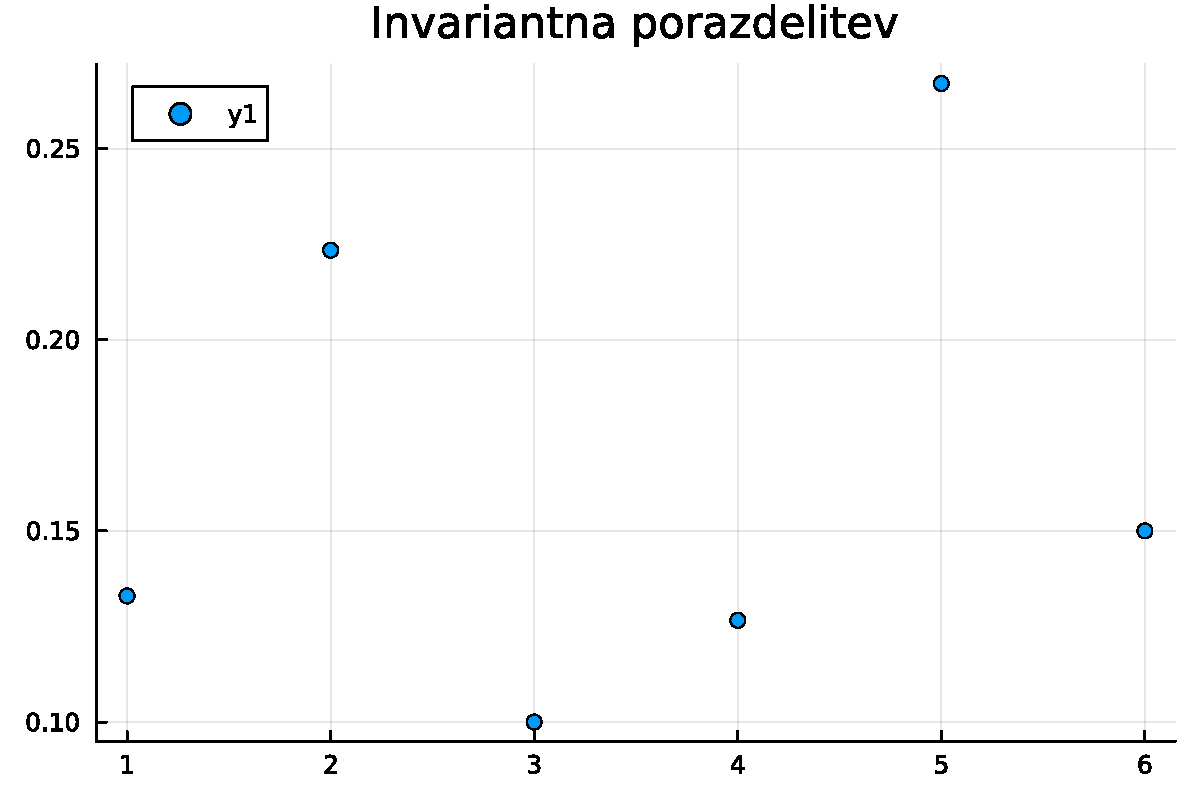
\includegraphics[width=\linewidth]{jl_Go6zFm/demo_3_1.pdf}


\end{document}
